\begin{figure}[H]
    \center
    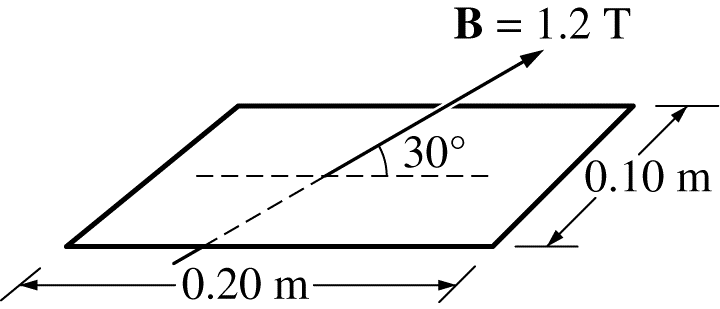
\includegraphics[scale=0.25]{images/img-005-013.png}
\end{figure}

% Multiple Choice Question 13
\begin{questions}\setcounter{question}{12}\question
A uniform magnetic field $\mathbf{B}$ of magnitude $1.2 \unit{T}$ passes through a rectangular loop of wire, which measures $0.10 \unit{m}$ by $0.20 \unit{m}$. The field is oriented $30^{\circ}$ with respect to the plane of the loop, as shown above. What is the magnetic flux through the loop?

\begin{oneparchoices}
\choice Zero
\choice $0.012 \unit{T \tightcdot m^2}$
\choice $0.020 \unit{T \tightcdot m^2}$
\choice $0.024 \unit{T \tightcdot m^2}$
\choice $0.048 \unit{T \tightcdot m^2}$
\end{oneparchoices}\end{questions}

